\section{Preface}
As discussed in previous articles, emerging blockchain technology is based on a series of rules and frameworks that try to look at what's going on inside the blocks and the process of building a block.
If a person sends a request on the network, the request will be verified by the network service providers or so-called nodes, then the request will be placed in the form of a transaction within a block.

\section{Definitions}

To begin to understand cryptocurrency, we have to examine the technology that powers it, and consequently, certain concepts to which cryptocurrency owes its existence. Let us first start by defining what cryptocurrency is. 


\subsection{Basic Definitions}

\begin{table}\centering
    \renewcommand{\arraystretch}{2.5}

    \begin{tabular}{@{}c|l@{}}
            \bfseries Phrase & implication\\
            \hline\hline
            Miner
            & 
            Transaction confirmer\\
            Public agreement
            &
            A V based method for accepting the transaction.
            \\
            Forking 
            & a fork is what happens when a blockchain diverges into two potential paths forward — 
            \\
             
            &
            either with regard to a network's transaction history or a new rule in deciding what makes 
            \\
            
            &
            a transaction valid. But forks also can be willingly introduced to the network.
            \\
            hash 
            &
            Applying hash is a way to check the accuracy of a transaction
            \\
            Node
            &
            A ledger in user side of block Chain.
            \\
            Time Stamp
            &
            Variables or variables to record time spent on blockchain
    \end{tabular}
\end{table}
\pagebreak

Table number one. An overview of widely used concepts 
\textcite{tasatanattakool2018blockchain}
\linebreak

\raggedright\subsection{General Definitions}
Blockchain:
A chain of blocks that each block contains valuable data without monitoring from the central server. This information is protected by encryption and cannot be changed.
Decentralized Blockchain:
Blockchain has a decentralized structure due to the lack of a central server.
Public Consensus:
Before new information is added to Blockchain, more than half of ninety people must confirm that this new information is valid for Blockchain.
Unchanging:
Once the information is added to the blockchain, it cannot be changed or deleted. The information is protected by blockchain, so the information is encrypted and makes it almost impossible to hack the information.
Extractor:
Users who use their computer power to extract blocks.

\section{Processes of Creating a blockchain }
Ethereum developer Vlad Zamfir says that cryptoeconomics is “A formal discipline that studies protocols that govern the production, distribution, and consumption of goods and services in a decentralized digital economy. Cryptoeconomics is a practical science that focuses on the design and characterization of these protocols.” The blockchain technology runs on the principles of cryptoeconomics as implied by the word Cryptoeconomics coming from the combination of Cryptography and Economics. The cryptoeconomy consists of cryptoeconomic approaches by combining cryptography and economics to create robust and decentralized Peer-to-Peer networks that thrive over time despite adversaries that attempt to disrupt the network. The cryptography underlying these systems is what makes the Peer-to- Peer communications within the networks secure and the economics are what incentivizes all actors to contribute to the network so that it thrives over time and to be applicable to traditional economic activities as well as newly created ones in terms of users, distributed capital markets, applications, services, micro payments, live collaboration, and auctions.\textcite{choecreating}
\subsection{Process 1: Create an address}

You need to have an address to connect to the ChinaBlock network. Creating an address is not difficult and time consuming, but it is necessary to connect to the network. Your URL consists of two parts, a public URL and a private URL, in which the URL is a URL that must be available to you and is your signature. Anyone with easy access to your private URL can do anything. Count on you, including stealing digital assets in that node.

\subsection{Process 2: Encryption}
Your request will be sent to the network with your signature (which is done via a private key) and this request will be verified through your public key, whether the request is digital currency transfer or just sending a text.
Whatever you want to do, it will be encrypted! If you want to send, for example, "Hello Sepehr" to someone, the word is encrypted through the hash pan and becomes a series of letters and meaningless numbers in the door. For example, "Hello Mohsen" becomes "bce9c72c24edbd3baa1d3cac4d457d45".
\newline

\centering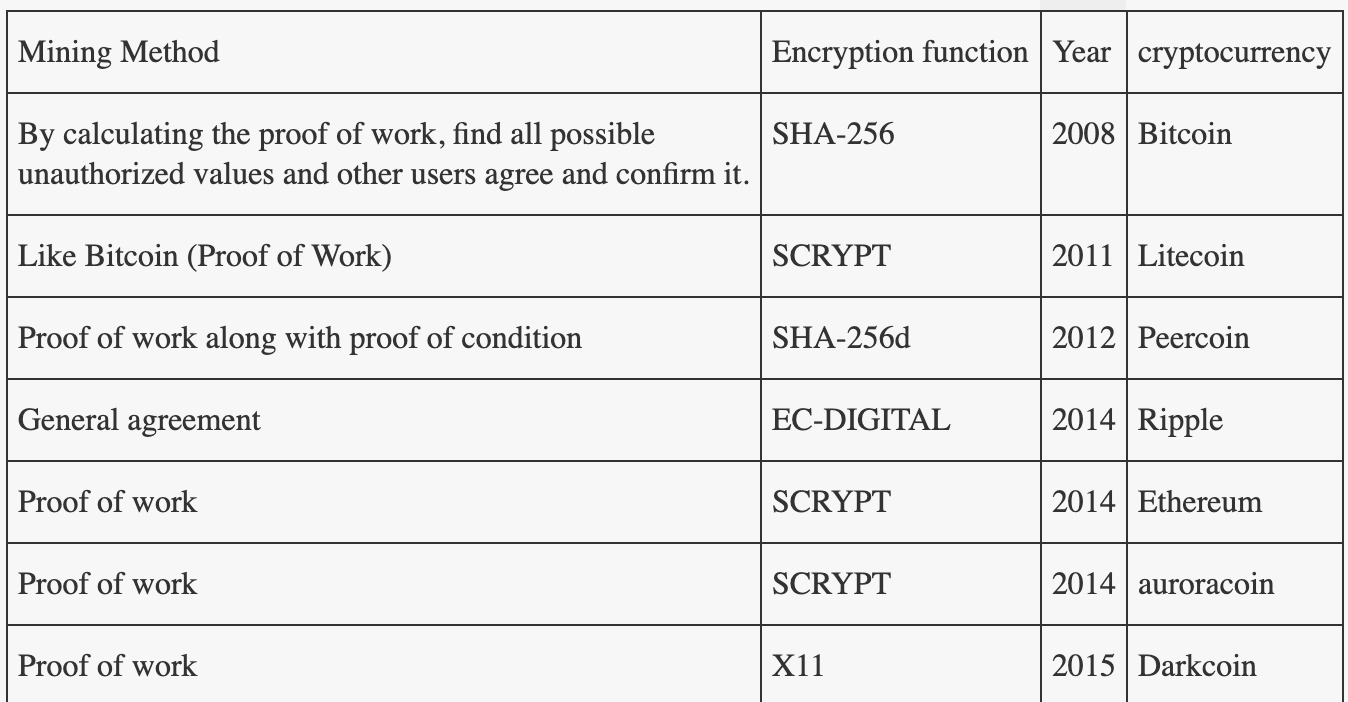
\includegraphics[width=15cm, height=7cm]{image/table2.png}
Table Two. General information about currency codes\textcite{tama2017critical}
\pagebreak
\begin{flushleft}
\subsection{Process 3: Prevent recurrent hashes}

The question may be, what if the same data is available? In the same way that the same hashes are created!
For example, consider a transaction with the same data being sent from one address to another, in which case duplicate hashes are generated, because everything is the same. The network has come up with a solution to this problem.
\section{Nonce}

Nans is made for this purpose, Nans is a random value that is added to the data and is created after the addition of a new hash, in which case the same data will not have the same hashes.
Process 5: Blockchain formation
In blockchain, each block depends on its previous block, so that when a series of transactions are placed in a block and in general that block is hash, this hash (which contains information from all previous transactions) is placed in the next block. Until the end…
• First of all, this is why they say the blockchain chain, because in each hash block there is a previous block and the chains are connected together.
• Secondly, this is why changing the information in each block causes the connection between the blocks to be disrupted, because even if the hash of a data change, the hash of all blocks changes.
This is not hidden from network members, so if someone wants to make a change, the network service providers will notice the change and will not approve it, unless 51 percent of the service providers accept the change and accept it.
According to the mentioned concepts, the level of security and transparency can be observed in the structure of "blockchain" and the way this network works can be interesting for those who are interested in its type.

\section{Data structure}

Deep and practical knowledge of data structure is essential when the goal is to become a blockchain developer. Blockchain developers are constantly displaying and optimizing existing data structures such as the Merkel Tree, the Petersia Tree, etc. to meet the needs of their personal network. Blockchain uses many data structures to build a secure and unchangeable system using advanced encryption. Knowledge of blockchain is incomplete without sufficient information about the structure of the data.

\section{Cryptography or encryption algorithm}

As mentioned earlier, blockchain is a combination of data structure and advanced encryption. Thus, it is clear that a good understanding of cryptography is essential for a blockchain developer. Many encryption methods, such as hash functions, such as SHA256 and KECCAK256, are used to generate digital signatures on blockchain instead of asymmetric encryption. Without an understanding of how they work, it becomes virtually impossible to develop a blockchain developer.

\section{Web Development}

Web development is a key aspect of blockchain development. When a person starts out as a blockchain developer in the industry, most of them are used for the initial design of applications and decentralized applications. This means that a blockchain developer must be familiar with the basic concepts of front-end user settings and back-end server side settings, such as creating interactive graphical user interfaces for Dapps, reviewing APIs, processing and processing requests, and more.

\section{Investigate the mathematics used in Bitcoin}

One of the reasons Bitcoin can be confusing for beginners is that Bitcoin technology offers a new definition of ownership. Traditionally, the owner has something like a house or some money, that is, he owns it or entrusts it to a trusted entity such as a bank.
The situation is different with Bitcoin. Bitcoin is not stored centrally or locally, so no institution is in charge. Bitcoin exists as a record in a distributed general ledger called a blockchain. The same versions of this Ledger are shared by a network of interconnected computers. Having bitcoin means being able to transfer control to another person. This is possible by creating a transfer history in the blockchain. But what makes it possible? The answer to this question is the accessibility of that pair of public and private ECDSA keys. What does this answer mean and how does it secure Bitcoin?
A closer look reveals that the ECDSA algorithm stands for Elliptic Curve Digital Signature Algorithm and means the digital signature algorithm based on the elliptical curve. ECDSA is a process that uses an elliptical curve and a finite field to sign information. Signing information in this algorithm is done in such a way that third parties can verify the validity of the signature, while only the signatory has the ability to create a signature. In the case of Bitcoin, the signed information is the transaction that transfers ownership.
The ECDSA algorithm has separate signature and verification procedures. Each procedure involves an algorithm consisting of several computational operations. The signature algorithm and the verification process use the private key and the public key, respectively. In the continuation of this article, we will give an example in this regard.

\subsection{Elliptical curves}
The elliptical curve is expressed as algebraic as follows:

\begin{equation}
y^2=x^3+ax+b
\end{equation}

If a is equal to zero and b is equal to 7 (the version used by Bitcoin) the share will be as follows:
\end{flushleft}
\centering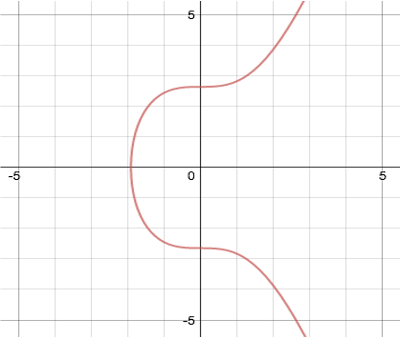
\includegraphics[width=8cm, height=6cm]{charts/1.png}

\begin{flushleft}
Elliptical curves have useful properties. For example, a nonlinear line that intersects two non-tangent points in a curve always passes through the third point on the curve. Another feature is that the non-vertical line tangent to the curve at one point intersects exactly another point on the curve. Using these features, we can define two other operations: adding a dot and doubling the coordinates of a point.\newline

Adding a point with the formula P + Q = R to achieve the x-axis coordinates is the third intersection point R on a line that includes P and Q. This definition is easier to understand as follows:
\end{flushleft}

\centering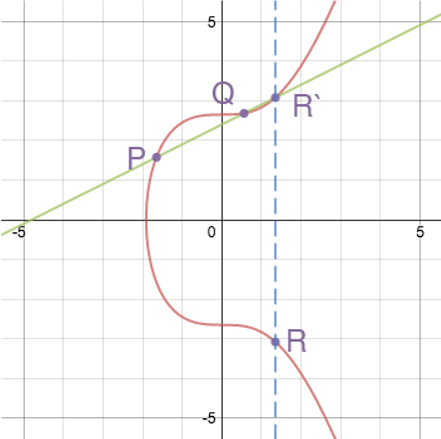
\includegraphics[width=8cm, height=6cm]{charts/2.png}

\begin{flushleft}
Doubling the coordinates of a point with the formula P + P = R and finding the line of tangent to the point whose coordinates are to be doubled and obtaining the coordinates of the x-axis is the intersection point R. Here's an example:

\end{flushleft}

\centering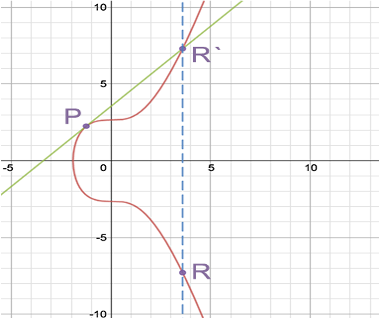
\includegraphics[width=8cm, height=6cm]{charts/3.png}

\begin{flushleft}
These two operations together to multiply the scalar by the formula R = a P and the sum of the point P with it are a. For example, we have:
\begin{equation}
R=7P,\newline
R=P+(P+(P+(P+(P+(P+P)))))
\end{equation}

The scalar multiplication process is usually made easier by combining point addition operations and doubling point coordinates. For example, we have:

\begin{equation}
R=7P,
R=P+6P,
R=P+2(P+2P)
\end{equation}

\subsection{Finite fields}
A finite field, in the context of ECDSA, can be thought of as a predefined range of positive numbers within which every calculation must fall. Any number outside this range “wraps around” so as to fall within the range.

The simplest way to think about this is calculating remainders, as represented by the modulus (mod) operator. For example, 9/7 gives 1 with a remainder of 2:

9 mod 7 = 2

Here our finite field is modulo 7, and all mod operations over this field yield a result falling within a range from 0 to 6.

\subsection{Putting it together}

ECDSA uses elliptic curves in the context of a finite field, which greatly changes their appearance but not their underlying equations or special properties. The same equation plotted above, in a finite field of modulo 67, looks like this:
\end{flushleft}
\centering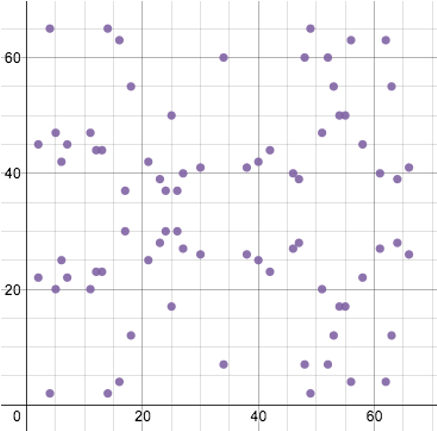
\includegraphics[width=8cm, height=6cm]{charts/4.png}

\begin{flushleft}
It’s now a set of points, in which all the x and y values are integers between 0 and 66. Note that the “curve” still retains its horizontal symmetry.

Point addition and doubling are now slightly different visually. Lines drawn on this graph will wrap around the horizontal and vertical directions, just like in a game of Asteroids, maintaining the same slope. So adding points (2, 22) and (6, 25) looks like this:
\end{flushleft}

\centering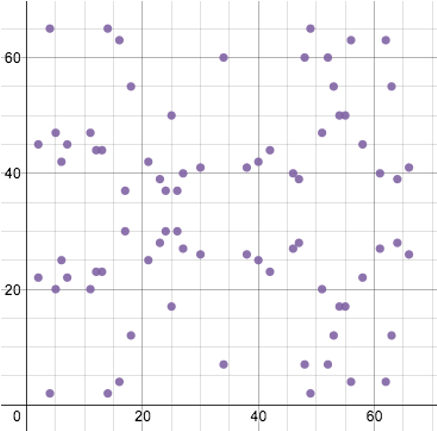
\includegraphics[width=8cm, height=6cm]{charts/4.png}

\begin{flushleft}
The third intersecting point is (47, 39) and its reflection point is (47, 28).

A protocol such as bitcoin selects a set of parameters for the elliptic curve and its finite field representation that is fixed for all users of the protocol. The parameters include the equation used, the prime modulo of the field, and a base point that falls on the curve. The order of the base point, which is not independently selected but is a function of the other parameters, can be thought of graphically as the number of times the point can be added to itself until its slope is infinite, or a vertical line. The base point is selected such that the order is a large prime number.

Bitcoin uses very large numbers for its base point, prime modulo, and order. In fact, all practical applications of ECDSA use enormous values. The security of the algorithm relies on these values being large, and therefore impractical to brute force or reverse engineer.

In the case of bitcoin:

Elliptic curve equation: 
\begin{equation}
y^2 = x^3 + 7
\end{equation}
Prime modulo = 2256 – 232 – 29 – 28 – 27 – 26 – 24 – 1 = FFFFFFFF FFFFFFFF FFFFFFFF FFFFFFFF FFFFFFFF FFFFFFFF FFFFFFFE FFFFFC2F
Who chose these numbers, and why? A great deal of research, and a fair amount of intrigue, surrounds the selection of appropriate parameters. After all, a large, seemingly random number could hide a backdoor method of reconstructing the private key. In brief, this particular realization goes by the name of secp256k1 and is part of a family of elliptic curve solutions over finite fields proposed for use in cryptography.



\subsection{Conclusion}

In this article, we explain the complex mathematical relationship between the public key and the private key. We have also seen how, even in the simplest of examples, the mathematical principles of signatures and verification become so complex. We accept this very complexity when the present parameters are 256-bit numbers. In this paper, we found that the clever use of the simplest mathematical procedures can create the necessary one-way path to maintain information asymmetry that defines bitcoin ownership. We have also regained the strength of this system, which includes completely secure protection of our private keys.
In other words, it is said that bitcoin is supported by mathematics. If you are interested in complex coding issues, we hope this article helps you take the next step in the discussion.\textcite{rykwalder_2014}

\section{Design}
Now, with the algorithms mentioned and the necessary processes in the blockchain, we examine the languages available for this purpose.g


\section{Choosing a programming Language}
If we want to become a blockchain developer, the first step is to choose a programming language that is determined by the type of project you have. In fact, there is no single programming language for blockchain programming, because as you change the way your project works, so does the programming language. For example, a person may choose the Python language to carry out their blockchain project, while another developer may use JavaScript.

So you need to first determine what digital currency can be the basic platform for your project, and you need to determine what you expect from the operation and purpose of that project. To view the best and most popular programming languages in 2020, you can use the articles published on IEEE and tiobe.com.
Accordingly, blockchain programming can be divided into 4 areas of work:
\begin{enumerate}
\item Creating and upgrading a blockchain network
\item Fabric hyperlink project to implement a decentralized general ledger
\item Launch an ICO
\item Build smart contracts and decentralized 
\end{enumerate}
programs (Dapp)
The first challenge is language security, programming. Because blockchain code is public and visible to all users, anyone can check the code and even make changes to it, so a hacker can infiltrate the network by finding security bugs. Steal millions of dollars or digital currency.
The second challenge is resource management. This means that the development of blockchain must be in line with the needs of the network. Because it is not possible to make the necessary predictions from the beginning of the project, it is best for the system to be prepared for questions from around the world or local questions. On the other hand, blockchain design should be the best way to create performance. Therefore, it will be important to use a flexible writing program that can run different instructions in parallel.

In the third challenge, the efficiency and performance of programming languages is assessed.
As mentioned, a blockchain should always display its highest capabilities. Therefore, the use of digital signatures improves the ability to parallelize the blockchain. You don't need anything more than a transaction, a signature, or a key to confirm a digital signature, and with these three confirmations, you can do the tasks in parallel. This feature is evident in all functions of a blockchain

\subsection{C++ Programming Language}
Language, C ++ Programming Program (C ++)
This language was developed by Strostrop more than 30 years ago. In addition to having all the key features of a C-programming language, such as flexibility, security, and efficiency, C ++ has tried to increase the concept of object-orientation. That's why C ++ is known as an object-oriented programming language, but C is a structured programming language.
Many Chinese blockchain developers are currently using the C ++ programming language to design the original ChinaClock core. However, due to the high dependence of C ++ on the type of old variables and commands, its use is not recommended for novice programmers. However, if you are proficient in using this programming language, you will gain a deep understanding of other programming languages.
Language J Java Program Writing
The Java programming language is the king of HTML / Css web pages, and is used to create high-security confidential blockchains because of its immutability, which prevents hacking and sabotage.

\subsection{Go(Language)
}
The Golang programming language, or GO for short, was created by Google in 2007, but over time, with the recognition of its performance in 2012, it was welcomed by the community of programmers. Go is a powerful, multi-purpose programming language that is simple, efficient, and secure. In addition, Go is an interpretive language and is able to work directly with operating systems. This feature has led to the use of this language in various areas of project development based on China.
Atrium SDK has now created a protocol based on the GO programming language, which is used to change a blockchain. The Linux Foundation also uses the Go language to develop high-tech fabric projects.

\subsection{Python Programming Language
}
Python was created by Guido van Rossum with the aim of creating simplicity and readability in the codes and commands of a language program. Many people who have just entered the world of "programming" are very interested in the Python language, because it is easy to learn and the language of "programming" is modern and efficient.
Although the Python language alone cannot create a blockchain-based structure, it must be said that in almost all blockchains, there is one or more general tools with or for Python.
\subsection{JavaScript 
}
JavaScript is the first programming language to be developed to create user interfaces and improve CTML and CSS pages. Today, almost all browsers support JavaScript well.
With the help of intermediaries such as animations, user menus, chat boxes, and interactive maps, Javascript has been able to evolve and improve the behavior of web pages in new and modern browsers. JavaScript is one of the languages of programming that is evolving and improving day by day and is relatively easy for beginners.
The use of JavaScript in blockchain-based projects was first used on the Lisk platform.
The developers of the Lisk project believe that JavaScript can implement a complete ecosystem on the blockchain. Therefore, the Lisk platform has made it possible for programmers to create and implement cloud-based programs in JavaScript.
Selection of auxiliary functions
Python is used to write this project. The reason for this choice is the existence of many libraries and additional auxiliary functions in this language, which speeds up the "writing program" operation. In this section, we will get acquainted with the components that help us.
\subsection{Sha encryption:
}
SHA-256 belongs to the SHA-2 Hash Encryption Functions family, designed by the NSA. Secure Hash Algorithms (SHA) is one of Hash's secure algorithms. Encrypted hash functions are a series of mathematical operations that are applied to digital data; a person can compare the hash calculated (output from the hash algorithm) with the amount of hashish expected of him / her, and can verify the accuracy of a data. Recognize. Data can be converted to hash in a one-way process, but the generated hash cannot be converted to primary data.
 The Sha-256 algorithm is based on the Merkle-Damgard structural method. Accordingly, the initial information is immediately divided into blocks, and after the changes that are made on it, the initial information becomes a 16-word output.
SHA-256 is used in various parts of the Bitcoin network: Extraction uses SHA-256 as a proof-of-work algorithm. SHA-256 is used to create Bitcoin addresses to improve security and privacy.

\subsection{Data conversion with Json:
}
JSON The acronym JavaScript Object Notation means "JavaScript object marking". Of course, don't pay too much attention to its meaning, because translating these phrases usually doesn't give a precise meaning.
Jason often uses a web server to send data to a web page.
Jason himself is self-describing Its codes are very easy due to the name / value structure.

\subsection{Sha encryption:
}
SHA-256 belongs to the SHA-2 Hash Encryption Functions family, designed by the NSA. Secure Hash Algorithms (SHA) is one of Hash's secure algorithms. Encrypted hash functions are a series of mathematical operations that are applied to digital data; a person can compare the hash calculated (output from the hash algorithm) with the amount of hashish expected of him / her, and can verify the accuracy of a data. Recognize. Data can be converted to hashes in a one-way process, but generated hashes cannot be converted to primary data.
 The Sha-256 algorithm is based on the Merkle-Damgard structural method. Accordingly, the initial information is immediately divided into blocks, and after the changes that are made on it, the initial information becomes a 16-word output.
SHA-256 is used in various parts of the Bitcoin network: Extraction uses SHA-256 as a proof-of-work algorithm. SHA-256 is used to create Bitcoin addresses to improve security and privacy.
Data conversion with Json:
JSON The acronym JavaScript Object Notation means "JavaScript object marking". Of course, don't pay too much attention to its meaning, because translating these phrases usually doesn't give a precise meaning.
Jason often uses a web server to send data to a web page.
Jason himself is self-describing, meaning that it's easy to understand its codes because of the name / value structure.

\subsection{Routing with Flask:
}
Flask is a Python-based web framework for creating fast and simple web servers developed by ArminerRunacher. Trying to simplify the design of the small and small frameworks and not giving many defaults to programmers is the reason why this package is called "software software". flask is free and open source and is licensed under the BSD.
Some of the strengths of Philosophy that encourage programmers to use are:
Flask is very easy to learn. If you're a little familiar with the Python language, you'll be able to get rid of it by looking at the code's code.
When working with Flask, you are free to do things as you wish. This means that this framework is quite flexible.
There is a strong community behind the Python language and the Philosophical Framework that you can count on when a problem arises.

\subsection{RSA encryption:
}
In all symmetric encryption algorithms with a symmetric key, the sender and receiver of the message must know the encryption key. When the sender of the message uses a unique, secret key for encryption, and the recipients of the message use the same key to decrypt it, disclosing the password via one of the recipients of the message endangers everyone's security. In such a situation, the sender will have to agree with each recipient individually on a symmetrical secret key so that each receiver has its own key and its disclosure does not interfere with the security of others. In this case, the sender of the message must define and hold the key to the number of recipients. Defining, for example, tens of thousands of symmetrical keys for users and storing and retrieving them safely is a big problem.
In public key algorithms, two completely different keys are used for encryption and decryption: "public key" and "private key".
The public key is used to encrypt information and everyone knows it, because this key is only used to encrypt information, and enemies will not be able to decrypt the data encrypted by others.
A private key is the key with which encrypted data is decrypted. No one, not even trustees and friends, knows this key. Thus, any network-level entity (whether user, machine, or process) needs two independent keys, only one of which is sensitive and secretive and must be carefully maintained. The nature of the encryption algorithm is such that in practice it is not possible to infer a private key by holding a public key.
In the following year, three people named Ryost, Shamir, and Adelman introduced an algorithm for implementing public key encryption with a pair of keys, known as RSA, which has been widely used over the last three decades and over time, optimized hardware and software. It was launched. Although a stronger algorithm called El Gamal was later developed, the RSA method is still at the top of the list of public key algorithms.
Suppose the sender of the pair message has an integer (e, n) as the public key to encrypt their information. On the opposite side, the receiver also uses a pair of numbers (d, n) to decrypt the message. Obviously, the two pairs of numbers (e, n) and (d, n) have a clever relationship with each other, but it is not possible to easily deduce d by having e and n. Assuming that such keys exist, the RSA algorithm Finally, the simplicity is as follows:
A) The message to be encrypted is divided into character K blocks (k bytes).
B) Each block is converted to an integer called Pi according to a completely arbitrary rule.
C) With the pair of numbers (e, n) for each Pi block, new numbers are obtained according to the following relation:
Ci = (Pi) e mod n
D) Ci codes are sent instead of the original Pi codes.
The method of decrypting the data is exactly the same as the encryption method, ie by having a pair of numbers (d, n), the encrypted blocks are decoded as follows. Should:
Pi = (Ci) d mod n
The whole algorithm ends here.
In RSA, the pair of numbers (e, n) with which the text is encrypted, the so-called public key, and the pair of numbers (d, n) through which the text is encrypted, the private key. Called. The basic point in RSA is that in order to ensure the inversion of the cryptographic method, the numbers must be true for the relation (x) e.d mod n = x, so care must be taken in the selection of numbers.
Another basic principle that must be followed in RSA encryption is that the Pi codes that we assign to each block must be in the 0 <= Pi <n condition. Therefore, if the blocks are modeled as k-bit strings, the 2K <n condition must be met. The reason for this is that it is easy to write the statement Pi mod n = Pi, otherwise, in general, this statement is not correct, and in this case, the correct decryption of the data will not be guaranteed.
The e and d selection methods proposed by RSA inventors are:
A) Two arbitrary (but large) numbers p and q are selected.
B) The numbers n and z are calculated according to the following two relations:
n = p * q
z = (p-1) * (q-1)
C) The number d is selected so that it is equal to the first z, meaning that no common factor is found on which both are divisible.
D) Based on d, the number e is selected so that the following relation is established: (In other words, the multiplicative multiplication of d in the measure of z is calculated and called e)
(e * d) mod z = 1
What is clear is that in practical applications, the numbers p and q are selected at least one hundred digits (one hundred digits in base ten), meaning that these two numbers are at least.. In this case, the correct number corresponding to the Pi blocks, which according to the above condition must be less than n, must not be more than 2 characters,
So each text block must have a maximum of 2 bits or 8 bits.
Here, it is necessary to note that in order to calculate Ae mod n, it is not necessary to multiply A by the number of e loads and then find its remainder on n, because using some mathematical properties, the result of the calculations never exceeds n.
Now suppose an intruder wants to get public by having the general key (e, n).. In this case, he must first decompose n into its first two factors, p and q, so that he can calculate z and Then he got d. There is no way to break down numbers into the first factor except by searching and testing, and given that n is at least two hundred digits, it will take thousands of years, even with the help of a computer.
Although research on the problem of decomposing large numbers into its factors is still ongoing, an efficient algorithm that can decompose large numbers at any time in fixed time or in small quantities has not yet been found. The year since the introduction of the RSA has not diminished its value, but only the keys have been enlarged to do so.
Since the first numbers have no known order, so choosing the first very large numbers p and q is one of the big challenges of RSA because to prove that a number like p is the first, the range of lesser or equal numbers p should be examined and p pivability studied.
The larger the p, the larger the search range .p. For example, the search range for numbers becomes 512 bit., Which makes it virtually impossible to search for such space. So the only solution is to use a series of mathematical theorems that help us narrow down the search range and reduce the guesswork.
\subsection{Binascii}
The binascii module includes a number of methods for converting between binary and different encrypted ASCII binary displays. Typically, you do not use these functions directly, but use packing modules.
\section{Conclusion:
}
According to the concepts, assumptions and study of all encryption algorithms required is the language that designed the existing algorithms in the simplest and fastest possible way. Python is a programming language that, with its rich and extensive libraries, speeds up project design faster and more powerfully.
\end{flushleft}
